% =============================================================
%  CS102-F26 Digital Design and Computer Architecture I
%  Lecture 01 -- The Essence of Computing (Unit 1)
%  Follows Chapter 1 of A Student's Computer Architecture Book I.
%
%  Build the slides and the print handout:  npm run materials -- lecture-01
% =============================================================
\documentclass{wosm-slides}
\usepackage{cs102-lectures}

\title[Lecture 01 \textperiodcentered\ The Essence of Computing]{The Essence of Computing}
\subtitle{Lecture 01: computation as change of state, and a short history of computing tools}

% ---------- Helpers for this lecture --------------------------
% A syllabus line: \unitline{3}{Boolean algebra}.
\newcommand*\unitline[2]{%
  \par\makebox[1.6em][r]{\ttfamily\color{wosm-muted}#1}\enspace#2}
\newcommand*\unitgroup[1]{%
  \par\vskip1pt{\ttfamily\scriptsize\color{wosm-accent}\MakeUppercase{#1}}\par}

% A timeline: \begin{timeline} \when{1642}{...} \end{timeline}
\newenvironment{timeline}
  {\par\smallskip
   \begin{tabular}{@{}>{\ttfamily\footnotesize\color{wosm-accent}}r
                   @{\hspace{0.9em}}>{\raggedright\arraybackslash}p{10.7cm}@{}}}
  {\end{tabular}\par}
\newcommand\when[2]{#1 & #2 \\ \addlinespace[0.35em]}

% Tally marks for the tally-counter states: \tally{3}.
\newcommand*\tally[1]{%
  \ifnum#1=0 \rule{0pt}{1em}\else
    \foreach \i in {1,...,#1}{\rule[-0.1em]{0.7pt}{1em}\hspace{2.5pt}}\unskip
  \fi}

% A row of switches, filled = on: \switches{0,1,1}.
\newcommand*\switches[1]{%
  \tikz[x=0.34cm, y=0.34cm, baseline=0.05cm]{%
    \foreach \b [count=\i] in {#1}{%
      \ifnum\b=1 \fill[wosm-text] (\i,0) rectangle ++(0.8,0.8);
      \else \draw[wosm-muted, line width=0.5pt] (\i+0.04,0.04) rectangle ++(0.72,0.72);
      \fi}}}

% One generation of the Game of Life on a 5 x 5 window:
% \lifegen{<generation>}{<live cells as column/row>}.
\newcommand*\lifegen[2]{%
  \begin{tikzpicture}[x=0.3cm, y=0.3cm]
    \draw[wosm-rule, line width=0.4pt] (-1,-1) grid (4,4);
    \foreach \c/\r in {#2}
      \fill[wosm-text] (\c+0.08,\r+0.08) rectangle ++(0.84,0.84);
    \node[below, inner sep=3pt] at (1.5,-1) {\wosmlabel{gen #1}};
  \end{tikzpicture}}

% =============================================================
\begin{document}

\maketitle

\begin{frame}{Today}
  \tableofcontents
\end{frame}

% =============================================================
\section{About this module}

\begin{frame}{From switches to a computer}
  This module shows how a computer is built, starting from nothing more than
  switches that are on or off. No prior knowledge of electronics is needed.

  \medskip
  \begin{columns}[T, totalwidth=\textwidth]
    \column{0.49\textwidth}
      \textbf{Part 1: the foundations}
      \begin{itemize}
        \item numeral systems
        \item Boolean algebra and Boolean functions
        \item logic gates
        \item combinational and sequential circuits
      \end{itemize}
    \column{0.49\textwidth}
      \textbf{Part 2: the computer}
      \begin{itemize}
        \item an instruction set architecture
        \item an arithmetic logic unit, registers and RAM
        \item a stepper and a controller
        \item all together: the \textbf{DX8}, a working 8-bit computer
      \end{itemize}
  \end{columns}

  \medskip
  \wosmlabel{Continued in Digital Design and Computer Architecture II (Semester 3).}
\end{frame}

\begin{frame}{The road map}
  \footnotesize
  \begin{columns}[T, totalwidth=\textwidth]
    \column{0.49\textwidth}
      \unitgroup{Foundations}
      \unitline{1}{\textcolor{wosm-accent}{\bfseries The essence of computing\quad$\leftarrow$ today}}
      \unitline{2}{Numeral systems}
      \unitline{3}{Boolean algebra: laws and theorems}
      \unitline{4}{Boolean functions: canonical forms}
      \unitline{5}{Karnaugh maps}
      \unitline{6}{Logic gates and universal gate sets}
      \unitgroup{Combinational circuits}
      \unitline{7}{Multiplexers and demultiplexers}
      \unitline{8}{Encoders, priority encoders and decoders}
      \unitline{9}{Timing of combinational circuits}
    \column{0.49\textwidth}
      \unitgroup{Sequential circuits}
      \unitline{10}{Finite state machines: Moore and Mealy}
      \unitline{11}{The clock; SR latch and D latch}
      \unitline{12}{Flip-flops: D, T and JK}
      \unitline{13}{Counters}
      \unitline{14}{Timing: setup and hold times}
      \unitgroup{Building the DX8}
      \unitline{15}{Instruction set architecture}
      \unitline{16}{Arithmetic: adders, two's complement}
      \unitline{17}{Logic and comparison}
      \unitline{18}{The arithmetic logic unit}
      \unitline{19}{Memory: registers, RAM, register file}
      \unitline{20}{Processor design}
      \unitline{21}{Stepper, data path and controller}
      \unitline{22}{Building and programming the DX8}
      \unitline{23}{Course review and exam}
  \end{columns}
\end{frame}

\begin{frame}{How the module works}
  \begin{columns}[T]
    \column{0.57\textwidth}
      \begin{itemize}
        \item Self-paced: all materials are on
          \href{https://moodle.wosm.academy/course/view.php?id=2}{Moodle}.
        \item Each week: two lectures, a central exercise with worked examples,
          and a tutorial in which the solutions of the week's exercise sheet are
          discussed.
        \item You build and test the circuits of every unit in the
          \textbf{Logisim-evolution} circuit simulator. Circuit files for the
          examples in the book are provided.
        \item Verilog models of many of the circuits are there if you want to go
          further.
      \end{itemize}
    \column{0.37\textwidth}
      \small
      \begin{tabular}{@{}lr@{}}
        \toprule
        Activity & Hours \\
        \midrule
        Lectures & 34 \\
        Labs and tutorials & 36 \\
        Independent study & 130 \\
        \midrule
        \textbf{Total} & \textbf{200} \\
        \bottomrule
      \end{tabular}

      \medskip
      \wosmlabel{7 ECTS credits}
  \end{columns}
\end{frame}

\begin{frame}{Assessment}
  \small
  \begin{tabular}{@{}llll@{}}
    \toprule
    Component & Weight & Due & Outcomes \\
    \midrule
    Quizzes & 20\% & throughout & LO1--LO5 \\
    Circuit-design project: the DX8 computer & 40\% & throughout & LO3--LO6 \\
    Final exam & 40\% & end of module & LO1--LO6 \\
    \bottomrule
  \end{tabular}

  \bigskip
  \normalsize
  \begin{itemize}
    \item In the project you build the DX8 computer, or an extension of it, in
      Logisim-evolution and run your own programs on it.
    \item Permitted support materials are provided in the exam; no other aids
      are allowed.
    \item Work submitted after the deadline is penalised.
    \item All submitted work must be your own: see the
      \href{https://wosm.academy/code-of-conduct/}{Code of Conduct}.
  \end{itemize}
\end{frame}

\begin{frame}{What you will be able to do}
  \small
  \begin{description}[LO6]
    \item[LO1] Represent numbers in binary, octal and hexadecimal, and convert
      between them.
    \item[LO2] Manipulate Boolean expressions, derive sum-of-products and
      product-of-sums forms, and simplify them with Karnaugh maps.
    \item[LO3] Implement Boolean functions with logic gates; design and analyse
      combinational circuits, including their delays.
    \item[LO4] Model sequential behaviour with Moore and Mealy machines; build
      latches, flip-flops, registers and counters; explain setup and hold times.
    \item[LO5] Explain the Von Neumann architecture and the role of an instruction
      set; design an ALU, a register file and byte-addressable memory.
    \item[LO6] Explain fetch, decode, execute and load; compare single-cycle,
      multi-cycle and pipelined designs; build and program a multi-cycle 8-bit
      computer in a circuit simulator.
  \end{description}
\end{frame}

\begin{frame}{Reading}
  \textbf{The book}\par\smallskip
  A.\ Khudiyev, \emph{A Student's Computer Architecture Book~I}, 2026. Free online
  at
  \href{https://alikhudiyev.com/courses/self-study/computer-architecture/tutorial/book/2026/05/12/computer-architecture-1.html}{alikhudiyev.com}.
  Circuit files and Verilog models:
  \href{https://github.com/AliKhudiyev/alikhudiyev.github.io/tree/main/assets/courses/comp-arch}{DX8 course material}.\par
  \smallskip
  \wosmlabel{Today: Chapter 1, The Essence of Computing}

  \bigskip
  \textbf{Recommended}\par\smallskip
  \small
  N.\ Nisan, S.\ Schocken, \emph{The Elements of Computing Systems}, 2nd ed., MIT
  Press, 2021.\par\smallskip
  S.\ L.\ Harris, D.\ Harris, \emph{Digital Design and Computer Architecture:
  RISC-V Edition}, Elsevier, 2022.\par\smallskip
  D.\ A.\ Patterson, J.\ L.\ Hennessy, \emph{Computer Organization and Design: The
  Hardware/Software Interface}.\par\smallskip
  C.\ Petzold, \emph{Code: The Hidden Language of Computer Hardware and Software},
  2nd ed., Microsoft Press, 2022.
\end{frame}

\begin{frame}{Getting help}
  \begin{tabular}{@{}>{\ttfamily\footnotesize\color{wosm-muted}}l@{\hspace{1.5em}}l@{}}
    Module leader & Dr.\ Ali Khudiyev \\[0.6em]
    Email & \href{mailto:ali.khudiyev@wosm.academy}{ali.khudiyev@wosm.academy} \\[0.6em]
    Office hours & Monday--Friday, 10:00--17:00 (Baku time, UTC+4) \\[0.6em]
    Course page & \href{https://moodle.wosm.academy/course/view.php?id=2}{moodle.wosm.academy} \\
  \end{tabular}
\end{frame}

% =============================================================
\section{What is computation?}

\begin{frame}{Computing before computers}
  Charles Babbage's Difference Engine and Analytical Engine, from the 1800s, are
  often called the very first computing devices. But the history of computing
  goes back much further:
  \begin{itemize}
    \item before Babbage, the abacus;
    \item long before the abacus, a bone with notches cut into it, used as early
      as 35,000~BCE;
    \item and before any tool, people counting and calculating in their heads.
  \end{itemize}

  \bigskip
  The same process can be carried out by a computer, a calculator, pen and paper,
  a notched bone, your fingers, or your imagination alone.

  \begin{block}{}
    Computing is not about the tools. It is about the \alert{process} that the
    tools carry out.
  \end{block}
\end{frame}

\begin{frame}{Tools and essence}
  \begin{columns}[T]
    \column{0.47\textwidth}
      \textbf{The tools}
      \begin{itemize}
        \item make computation \alert{efficient}: how fast it is, and how much
          energy it takes
        \item keep changing: notches, beads, gears, relays, vacuum tubes,
          transistors
      \end{itemize}
    \column{0.47\textwidth}
      \textbf{The essence}
      \begin{itemize}
        \item is the process itself
        \item stays the same, whatever the tool
        \item sets the rules that every tool has to follow
      \end{itemize}
  \end{columns}

  \bigskip
  \begin{remark}
    This module studies both: the essence (Boolean algebra, state machines) and one
    family of tools built on it (digital circuits).
  \end{remark}
\end{frame}

\begin{frame}{Computation without people}
  Imagine looking at the Earth from space, with no people on it. You would still
  see
  \begin{itemize}
    \item the planet moving and the weather changing,
    \item trees growing, bees flying, animals fighting,
    \item waves colliding.
  \end{itemize}
  Each of these processes moves the world from one \alert{state} into another.

  \bigskip
  \begin{block}{The view of this module}
    Changing from one state to the next takes some energy. In computer science we
    see this change of state as the computation itself.
  \end{block}
\end{frame}

\begin{frame}{State and computation}
  \begin{definition}[State]
    The \emph{state} of a system is what we need to know about it at one moment to
    say, given the rules and the inputs, what it will do next.
  \end{definition}

  \begin{definition}[Computation]
    A \emph{computation} is a sequence of changes of state, in which each next
    state follows from the current state, and the input, by fixed rules.
  \end{definition}

  Neither definition mentions a tool: the same rules can be followed in your head,
  with pen and paper, or by a machine.
\end{frame}

\begin{frame}{Example: adding with pen and paper}
  Compute $47 + 38$, one column at a time, from the right.

  \medskip
  \begin{columns}[T, totalwidth=\textwidth]
    \column{0.42\textwidth}
      \begin{tabular}{@{}lll@{}}
        \toprule
        Step & Written so far & Carry \\
        \midrule
        0 & (nothing) & 0 \\
        1 & 5 & 1 \\
        2 & 85 & 0 \\
        \bottomrule
      \end{tabular}
    \column{0.54\textwidth}
      \begin{itemize}
        \item State: the digits written so far, and the carry.
        \item Rule: add the two digits of the next column and the carry; write the
          last digit of the sum, carry the rest.
        \item Step 1: $7 + 8 + 0 = 15$. Step 2: $4 + 3 + 1 = 8$.
      \end{itemize}
  \end{columns}

  \bigskip
  The adders we build later work the same way, in binary: column by column,
  passing a carry along \unitref{16}.
\end{frame}

\begin{frame}{The simplest computation: a tally}
  Count the days by cutting one more notch into a bone every day.

  \bigskip
  \begin{center}
  \begin{tikzpicture}[node distance=1.25cm]
    \node[box] (s0) {\tally{0}};
    \node[box, right=of s0] (s1) {\tally{1}};
    \node[box, right=of s1] (s2) {\tally{2}};
    \node[box, right=of s2] (s3) {\tally{3}};
    \node[right=0.9cm of s3] (more) {\dots};
    \foreach \a/\b in {s0/s1, s1/s2, s2/s3, s3/more}
      \draw[arrow] (\a) -- node[above, edgelabel] {a day} (\b);
    \foreach \n/\k in {s0/0, s1/1, s2/2, s3/3}
      \node[below=2pt of \n, edgelabel] {\k\ days};
  \end{tikzpicture}
  \end{center}

  \bigskip
  \begin{itemize}
    \item State: the number of notches. Rule: one more notch per day.
    \item The same computation runs on a bone, on your fingers, in your head, or in
      a counter circuit \unitref{13}.
  \end{itemize}
\end{frame}

\begin{frame}{Current state, input, next state}
  The next state is a function of the current state and the input:
  $s_{t+1} = f(s_t,\, x_t)$.

  \smallskip
  \begin{columns}[T, totalwidth=\textwidth]
    \column{0.42\textwidth}
      \wosmlabel{A lamp with a push button}\par\smallskip
      \small
      \begin{tabular}{@{}lll@{}}
        \toprule
        State $s_t$ & Input $x_t$ & Next $s_{t+1}$ \\
        \midrule
        off & none & off \\
        off & press & on \\
        on & none & on \\
        on & press & off \\
        \bottomrule
      \end{tabular}
    \column{0.56\textwidth}
      \centering
      \begin{tikzpicture}[every loop/.style={arrow, looseness=6}]
        \node[st] (off) {off};
        \node[st, right=1.8cm of off] (on) {on};
        \draw[arrow] (off) to[bend left=30] node[above, edgelabel] {press} (on);
        \draw[arrow] (on) to[bend left=30] node[below, edgelabel] {press} (off);
        \draw (off) edge[loop left] node[left, edgelabel] {none} (off);
        \draw (on) edge[loop right] node[right, edgelabel] {none} (on);
      \end{tikzpicture}
  \end{columns}

  \begin{remark}[Coming back]
    Finitely many states and a rule like this make a finite state machine
    \unitref{10}. The lamp's on/off memory, built from gates, is a T flip-flop
    \unitref{12}.
  \end{remark}
\end{frame}

\begin{frame}{Our logo is a computation}
  \small
  In Conway's \emph{Game of Life} (1970) the state is a grid of cells, each alive
  or dead. At every step, all cells change at once, by looking at their 8
  neighbours:
  \begin{itemize}
    \item a live cell with 2 or 3 live neighbours stays alive; every other live
      cell dies;
    \item a dead cell with exactly 3 live neighbours comes alive.
  \end{itemize}

  \medskip
  \begin{center}
    \lifegen{0}{0/0, 1/0, 2/0, 2/1, 1/2}\hspace{0.7cm}%
    \lifegen{1}{0/1, 1/-1, 1/0, 2/0, 2/1}\hspace{0.7cm}%
    \lifegen{2}{0/0, 1/-1, 2/-1, 2/0, 2/1}\hspace{0.7cm}%
    \lifegen{3}{1/-1, 1/1, 2/-1, 2/0, 3/0}\hspace{0.7cm}%
    \lifegen{4}{1/-1, 2/-1, 2/1, 3/-1, 3/0}
  \end{center}

  After 4 steps the \emph{glider} has its original shape again, one cell further
  along the diagonal. Generation~0 is the mark on every one of these slides.\par
  \smallskip
  \wosmlabel{In Life, isolated cells starve and cells in company survive.}
\end{frame}

\begin{frame}{How many states?}
  A row of switches, each on or off. How many different states can the row be in?

  \bigskip
  \begin{columns}[T]
    \column{0.4\textwidth}
      \begin{tabular}{@{}lr@{}}
        \toprule
        Switches & States \\
        \midrule
        1 & \uncover<2->{2} \\
        2 & \uncover<3->{4} \\
        3 & \uncover<4->{8} \\
        $n$ & \uncover<5->{$2^n$} \\
        \bottomrule
      \end{tabular}
    \column{0.5\textwidth}
      \uncover<4->{%
        \wosmlabel{The 8 states of 3 switches (filled = on)}\par\medskip
        \begin{tabular}{@{}ll@{}}
          \switches{0,0,0} & \switches{1,0,0} \\[2pt]
          \switches{0,0,1} & \switches{1,0,1} \\[2pt]
          \switches{0,1,0} & \switches{1,1,0} \\[2pt]
          \switches{0,1,1} & \switches{1,1,1} \\
        \end{tabular}}
  \end{columns}

  \bigskip
  \uncover<5->{Each extra switch doubles the number of states. Naming these states
  with numbers is the topic of the next lecture: numeral systems, and binary in
  particular \unitref{2}.}
\end{frame}

% =============================================================
\section{A short history of computing tools}

\begin{frame}{Counting by hand}
  \begin{timeline}
    \when{c.\ 35,000 BCE}{The \textbf{Lebombo bone}: an 8\,cm piece of baboon
      fibula with notches cut into it, believed to have been used to count days
      and track time (its purpose is debated).}
    \when{antiquity}{The \textbf{abacus}: counters on lines or rods. Where a counter
      sits says what it is worth, an idea we meet again in positional numeral
      systems \unitref{2}.}
    \when{2nd--1st c.\ BCE}{The \textbf{Antikythera mechanism}: bronze gear wheels
      that predict the positions of the Sun and the Moon, and eclipses.}
  \end{timeline}

  \smallskip
  The tools for computing may have started then. The essence of computing was there
  long before: people counted and calculated in their heads.
\end{frame}

\begin{frame}{Machines that calculate}
  \begin{timeline}
    \when{1642}{Blaise Pascal's calculator adds and subtracts with gear wheels; a
      carry passes from one wheel to the next.}
    \when{1670s--1690s}{Gottfried Wilhelm Leibniz's stepped reckoner also
      multiplies and divides.}
    \when{1703}{Leibniz publishes his account of \textbf{binary} arithmetic: every
      number written with the digits 0 and 1 only.}
    \when{1804}{Joseph Marie Jacquard's loom: \textbf{punched cards} choose the
      pattern it weaves. Change the cards, and the same machine weaves something
      else.}
    \when{1822}{Charles Babbage proposes the \textbf{Difference Engine}.}
  \end{timeline}
\end{frame}

\begin{frame}{Babbage's engines}
  \begin{itemize}
    \item The \textbf{Difference Engine} (1822) computes tables of polynomials
      automatically, using addition only.
    \item The \textbf{Analytical Engine} (designed from 1837) is general-purpose.
      It is programmed with punched cards, as Jacquard's loom is, and has a
      \emph{mill} that calculates and a \emph{store} that holds numbers: today we
      say processor and memory.
    \item In 1843 Ada Lovelace publishes notes with a method for computing
      Bernoulli numbers on the Analytical Engine, often called the first computer
      program.
  \end{itemize}

  \begin{remark}
    Neither engine was finished in Babbage's lifetime. In 1991 the Science Museum
    in London completed his Difference Engine No.~2 from his drawings. It works.
  \end{remark}
\end{frame}

\begin{frame}{The method of differences}
  How can a machine that can only add compute $n^2$?

  \medskip
  \begin{center}
    \renewcommand{\arraystretch}{1.25}
    \begin{tabular}{@{}l*{11}{c}@{}}
      $n$          & 0 && 1 && 2 && 3 && 4 && \uncover<2->{5} \\
      $n^2$        & 0 && 1 && 4 && 9 && 16 && \uncover<2->{\alert{25}} \\
      first diff.  && 1 && 3 && 5 && 7 && \uncover<2->{\alert{9}} & \\
      second diff. &&& 2 && 2 && 2 && \uncover<2->{\alert{2}} && \\
    \end{tabular}
  \end{center}

  \uncover<2->{The second differences are always 2. Work upwards from them:
  $7 + 2 = 9$, then $16 + 9 = 25$. Two additions per new value, and no
  multiplication.}
\end{frame}

\begin{frame}{The method of differences as a computation}
  \begin{itemize}
    \item State: the pair $(v, d)$, the current value and its difference.
    \item Rule: $v \leftarrow v + d$, then $d \leftarrow d + 2$.
  \end{itemize}

  \medskip
  \begin{center}
    $(0,1) \to (1,3) \to (4,5) \to (9,7) \to (16,9) \to (25,11) \to \cdots$
  \end{center}

  \medskip
  \begin{remark}
    A polynomial of degree $k$ has constant $k$-th differences, so $k$ additions
    per step are enough. Difference Engine No.~2 works with seven orders of
    differences on 31-digit numbers.
  \end{remark}
\end{frame}

\begin{frame}{From gears to switches}
  \begin{timeline}
    \when{1854}{George Boole, \emph{An Investigation of the Laws of Thought}: an
      algebra of true and false \unitref{3}.}
    \when{1936}{Alan Turing defines computation precisely: a machine in one of
      finitely many states reads and writes symbols on a tape, following fixed
      rules.}
    \when{1937}{Claude Shannon shows that Boolean algebra describes circuits of
      relays and switches \unitref{3--6}.}
    \when{1945}{ENIAC: electronic, with about 18,000 vacuum tubes. John von
      Neumann's report on the EDVAC: program and data in the same memory
      \unitref{15}.}
  \end{timeline}
\end{frame}

\begin{frame}{From switches to chips}
  \begin{timeline}
    \when{1947}{The \textbf{transistor} (Bell Labs): a small, fast and reliable
      electronic switch.}
    \when{1958--59}{The \textbf{integrated circuit} (Jack Kilby, Robert Noyce):
      many transistors on a single chip.}
    \when{1971}{The Intel 4004, the first commercial \textbf{microprocessor}: a
      4-bit processor on one chip, with about 2,300 transistors.}
    \when{today}{A phone processor has billions of transistors.}
    \when{this module}{The \textbf{DX8}: an 8-bit computer that you build yourself.}
  \end{timeline}

  \bigskip
  You may be reading this on a computer, a phone or even a smart watch. Imagine how
  that would have looked to the people who cut notches into bones.
\end{frame}

\begin{frame}{Same essence, better tools}
  \begin{center}
    \small
    fingers $\rightarrow$ notched bone $\rightarrow$ abacus $\rightarrow$
    gears $\rightarrow$ punched cards $\rightarrow$ relays $\rightarrow$
    vacuum tubes $\rightarrow$ transistors $\rightarrow$ chips
  \end{center}

  \bigskip
  \begin{itemize}
    \item The tools became faster, smaller and cheaper, and use less energy: they
      became more \alert{efficient}.
    \item The essence did not change: a state, and rules that change it.
    \item From Boole and Shannon on, the rules are Boolean algebra and the tool is a
      switch that is on or off. This whole module is built on that.
  \end{itemize}

  \bigskip
  \begin{block}{}
    We have come a long way. The task now is to understand this long history, and
    to push it further than where it stands today.
  \end{block}
\end{frame}

% =============================================================
\section{Building a computer}

\begin{frame}{Layers of abstraction}
  \begin{columns}[T]
    \column{0.6\textwidth}
      \begin{tikzpicture}
        \foreach \text/\units [count=\i from 0] in {
            {Switches: on or off}/1,
            {Numbers in binary}/2,
            {Boolean algebra and Boolean functions}/3--5,
            {Logic gates}/6,
            {Combinational circuits}/7--9,
            {Sequential circuits}/10--14,
            {ALU, registers and RAM}/15--19,
            {The processor: stepper and controller}/20--21,
            {The DX8, running your programs}/22} {
          \draw[wosm-rule, fill=wosm-box] (0,0.58*\i) rectangle ++(7.4,0.5);
          \node[anchor=west, font=\footnotesize] at (0.1,0.58*\i+0.25) {\text};
          \node[anchor=east] at (7.3,0.58*\i+0.25) {\wosmlabel{\units}};
        }
      \end{tikzpicture}
    \column{0.36\textwidth}
      \begin{itemize}
        \item Each layer is built only from the layer below it.
        \item Each layer hides the details of the layer below from the layer above.
        \item This is how a system with millions of parts stays understandable.
      \end{itemize}
      \medskip
      \wosmlabel{Numbers on the right: units}
  \end{columns}
\end{frame}

\begin{frame}{What does it take to build a computer?}
  About 70 pages of the book to learn the fundamentals, and then about 15 pages to
  put everything together.

  \bigskip
  \begin{tabular}{@{}lll@{}}
    \toprule
    Chapter & & Units \\
    \midrule
    1 & The Essence of Computing & 1 \\
    2 & Foundations \& Boolean Algebra & 2--5 \\
    3 & Logic Gates \& Circuits & 6 \\
    4 & Combinational Logic & 7--9 \\
    5 & Sequential Logic & 10--14 \\
    6 & Let's Build a Computer! & 15--22 \\
    7 & Epilogue & \\
    \bottomrule
  \end{tabular}
\end{frame}

\begin{frame}{Where we are going: the DX8}
  \begin{center}
    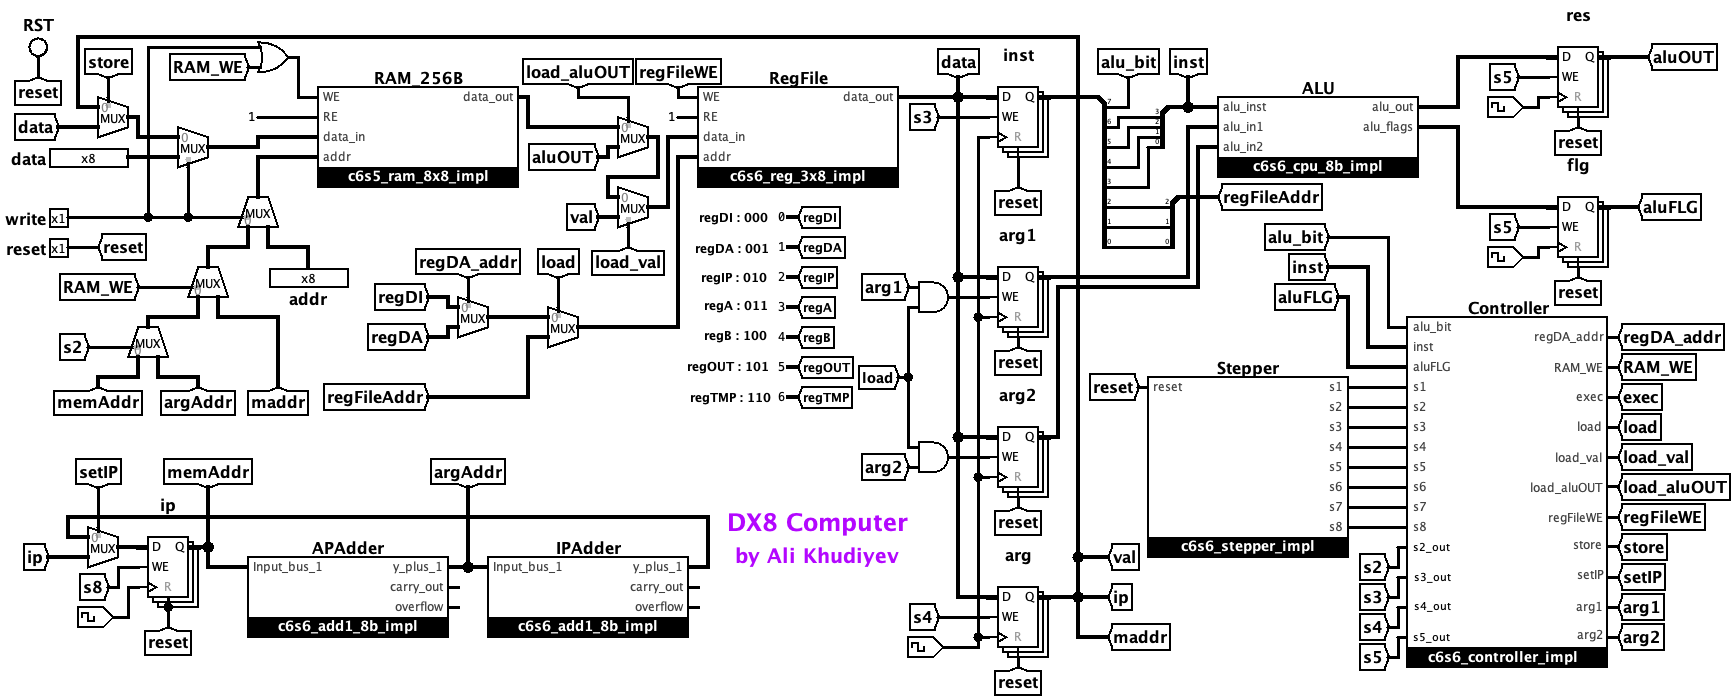
\includegraphics[width=0.97\linewidth]{figures/dx8.png}
  \end{center}
  \vspace{-0.6em}
  \wosmlabel{The DX8 computer in Logisim-evolution, from Chapter 6 of the book.}
\end{frame}

\begin{frame}{The DX8 at a glance}
  \begin{columns}[T]
    \column{0.47\textwidth}
      \begin{itemize}
        \item an 8-bit computer
        \item instructions of 16 bits (2 bytes)
        \item a register file of 8 registers, selected by 3-bit addresses
        \item $2^8 = 256$ bytes of RAM
      \end{itemize}
    \column{0.47\textwidth}
      \begin{itemize}
        \item an arithmetic logic unit (ALU)
        \item a stepper and a controller that drive every step, in time with the
          clock
        \item each instruction runs in four stages: fetch, decode, execute and load
      \end{itemize}
  \end{columns}

  \bigskip
  Every part of it is made of the circuits of Units 6--14, which are made of logic
  gates, which are made of switches.
\end{frame}

% =============================================================
\section{Summary}

\begin{frame}{Summary}
  \begin{itemize}
    \item Computation is a change of state that follows rules. It does not depend
      on the tool that carries it out.
    \item The state, the input and a rule give the next state:
      $s_{t+1} = f(s_t, x_t)$.
    \item Tools make computation efficient. From notched bones to chips with
      billions of transistors, the tools changed; the essence did not.
    \item Boolean algebra and on/off switches are the foundation of this module.
    \item We will build the DX8 computer layer by layer, from switches up.
  \end{itemize}
\end{frame}

\begin{frame}{Before the next lecture}
  \begin{itemize}
    \item Read Chapter~1 of the book, \emph{The Essence of Computing}.
    \item Install \href{https://github.com/logisim-evolution/logisim-evolution}{Logisim-evolution}
      (free), the circuit simulator for the exercises.
    \item Think of three processes around you. For each: what is the state, what
      changes it, and which tool, if any, carries it out?
  \end{itemize}

  \begin{block}{Next lecture \unitref{2}}
    Numeral systems, additive and positional; binary, octal and hexadecimal.
  \end{block}
\end{frame}

\end{document}
